\documentclass[10pt]{beamer}
\usetheme[
%%% option passed to the outer theme
%    progressstyle=fixedCircCnt,   % fixedCircCnt, movingCircCnt (moving is deault)
  ]{Feather}
  
% If you want to change the colors of the various elements in the theme, edit and uncomment the following lines

% Change the bar colors:
%\setbeamercolor{Feather}{fg=red!20,bg=red}

% Change the color of the structural elements:
%\setbeamercolor{structure}{fg=red}

% Change the frame title text color:
%\setbeamercolor{frametitle}{fg=blue}

% Change the normal text color background:
%\setbeamercolor{normal text}{fg=black,bg=gray!10}

%-------------------------------------------------------
% INCLUDE PACKAGES
%-------------------------------------------------------
\usepackage{subfig}
\usepackage[utf8]{inputenc}
\usepackage[spanish]{babel}
\usepackage[T1]{fontenc}
\usepackage{helvet}
\setbeamertemplate{caption}[numbered]
\setbeamertemplate{frametitle continuation}{} %continuation of frames
\bibstyle

% Another Packages

\usepackage{array}
\usepackage{float}
\usepackage{multirow}
\usepackage{amssymb}
\usepackage{graphicx}

% Tikz

\usepackage{tikz}
\usetikzlibrary{mindmap}
\definecolor{myblue}{HTML}{020364}
\usetikzlibrary{shapes,arrows,matrix,decorations.pathreplacing,shapes.geometric,positioning}  
% Gantt
\usepackage{pgfgantt}
\usepackage{adjustbox} %Ajustar a la página

% Items

\usepackage{enumitem}
\usepackage{amsfonts}

%videos

%\usepackage{media9}
\usepackage{multimedia}

% No numbering in references

%\newcommand{\backupbegin}{
%   \newcounter{framenumberappendix}
%   \setcounter{framenumberappendix}{\value{framenumber}}
%}
%\newcommand{\backupend}{
%   \addtocounter{framenumberappendix}{-\value{framenumber}}
%   \addtocounter{framenumber}{\value{framenumberappendix}} 
%}

%-------------------------------------------------------
% DEFFINING AND REDEFINING COMMANDS
%-------------------------------------------------------

% colored hyperlinks
\newcommand{\chref}[2]{
  \href{#1}{{\usebeamercolor[bg]{Feather}#2}}
}

%-------------------------------------------------------
% INFORMATION IN THE TITLE PAGE
%-------------------------------------------------------

\title[Passive Dynamic System for Energy Returning on Transtibial Prosthesis] % [] is optional - is placed on the bottom of the sidebar on every slide
{ % is placed on the title page
      \textbf{Passive Dynamic System for Energy Returning on Transtibial Prosthesis}
}

\author[Edwin N. Prieto]
{      Nikolay Prieto PhD(c). \\
      {\ttfamily enprietop@unal.edu.co}
}

\institute[]
{
      Doctorate in Engineering - Mechanics and Mechatronics Department\\
      School of Engineering\\
      Universidad Nacional de Colombia Bogotá\\
  
  %there must be an empty line above this line - otherwise some unwanted space is added between the university and the country (I do not know why;( )
}

\date{\today}

%-------------------------------------------------------
% THE BODY OF THE PRESENTATION
%-------------------------------------------------------

\begin{document}

%-------------------------------------------------------
% THE TITLEPAGE
%-------------------------------------------------------

{\BiOM% % this is the name of the PDF file for the background
\begin{frame}[plain,noframenumbering] % the plain option removes the header from the title page, noframenumbering removes the numbering of this frame only
  \titlepage % call the title page information from above
\end{frame}}


\begin{frame}[noframenumbering]{Outline}{}
\tableofcontents[
sectionstyle=show/show,
subsectionstyle=hide/hide/hide,
] 
\end{frame}

\AtBeginSection[]{

  \frame<beamer>[noframenumbering]{ 

    \frametitle{Índice}   

    \tableofcontents[
currentsection,
sectionstyle=show/shaded,
subsectionstyle=hide/hide/hide
] 
  }
}

\section{Motivation}
\begin{frame}{Recent Advances in Commercial Prosthesis}

\begin{figure}
\begin{centering}
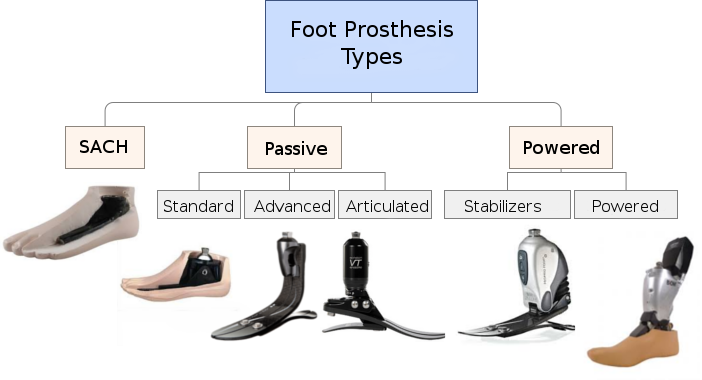
\includegraphics[scale=0.38]{Feathergraphics/GeneracionesprotesisEng}
\par\end{centering}
\caption{{\footnotesize{}Commercial prosthesis classes grouping. Adapted from Cherelle \emph{et al.} \cite{Cherelle2014a}} }

\end{figure}

\end{frame}

\begin{frame}{Energy Returning Principle}

\begin{figure}
\begin{centering}
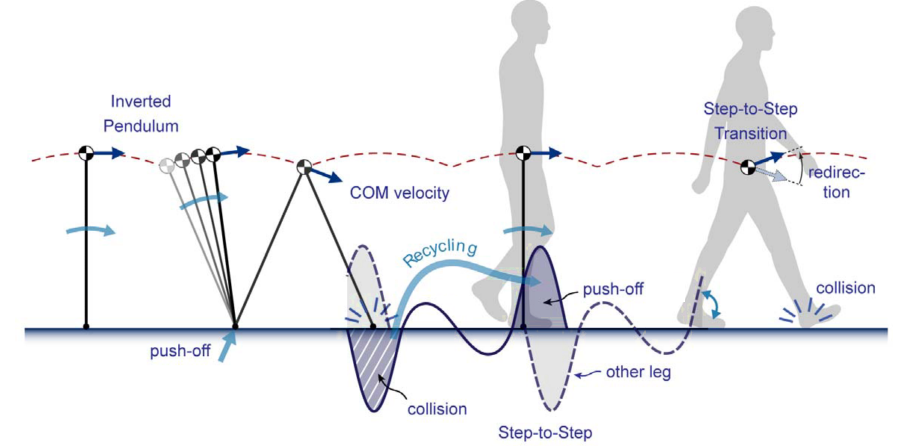
\includegraphics[scale=0.30]{Feathergraphics/RecycledEng}
\par\end{centering}

{\footnotesize \caption{\label{fig:Representaci} The leg in stance behaves similar to an inverted pendulum, supporting the body CoM until the other leg contacts the ground and mechanical energy is dissipated, then the vector velocity of the CoM is redirected. Figure modified from Collins and Kuo\cite{Collins2010}.}}

\end{figure}

\end{frame}



\begin{frame}{Principles of Prosthetic Feet}
\begin{alertblock}{}

\begin{itemize}
\item {Stiffness/flexibility.}
\item {Damping.}
\item {Roll-Over characteristics.}
\item {Active push-off in late stance phase.}
\item {Toe clearance during swing phase}
\end{itemize}
\end{alertblock}
\end{frame}

\begin{frame}{The Ankle Dynamic Joint Stiffness (DJS)}

\begin{figure}[h]
\begin{center}
\centerline{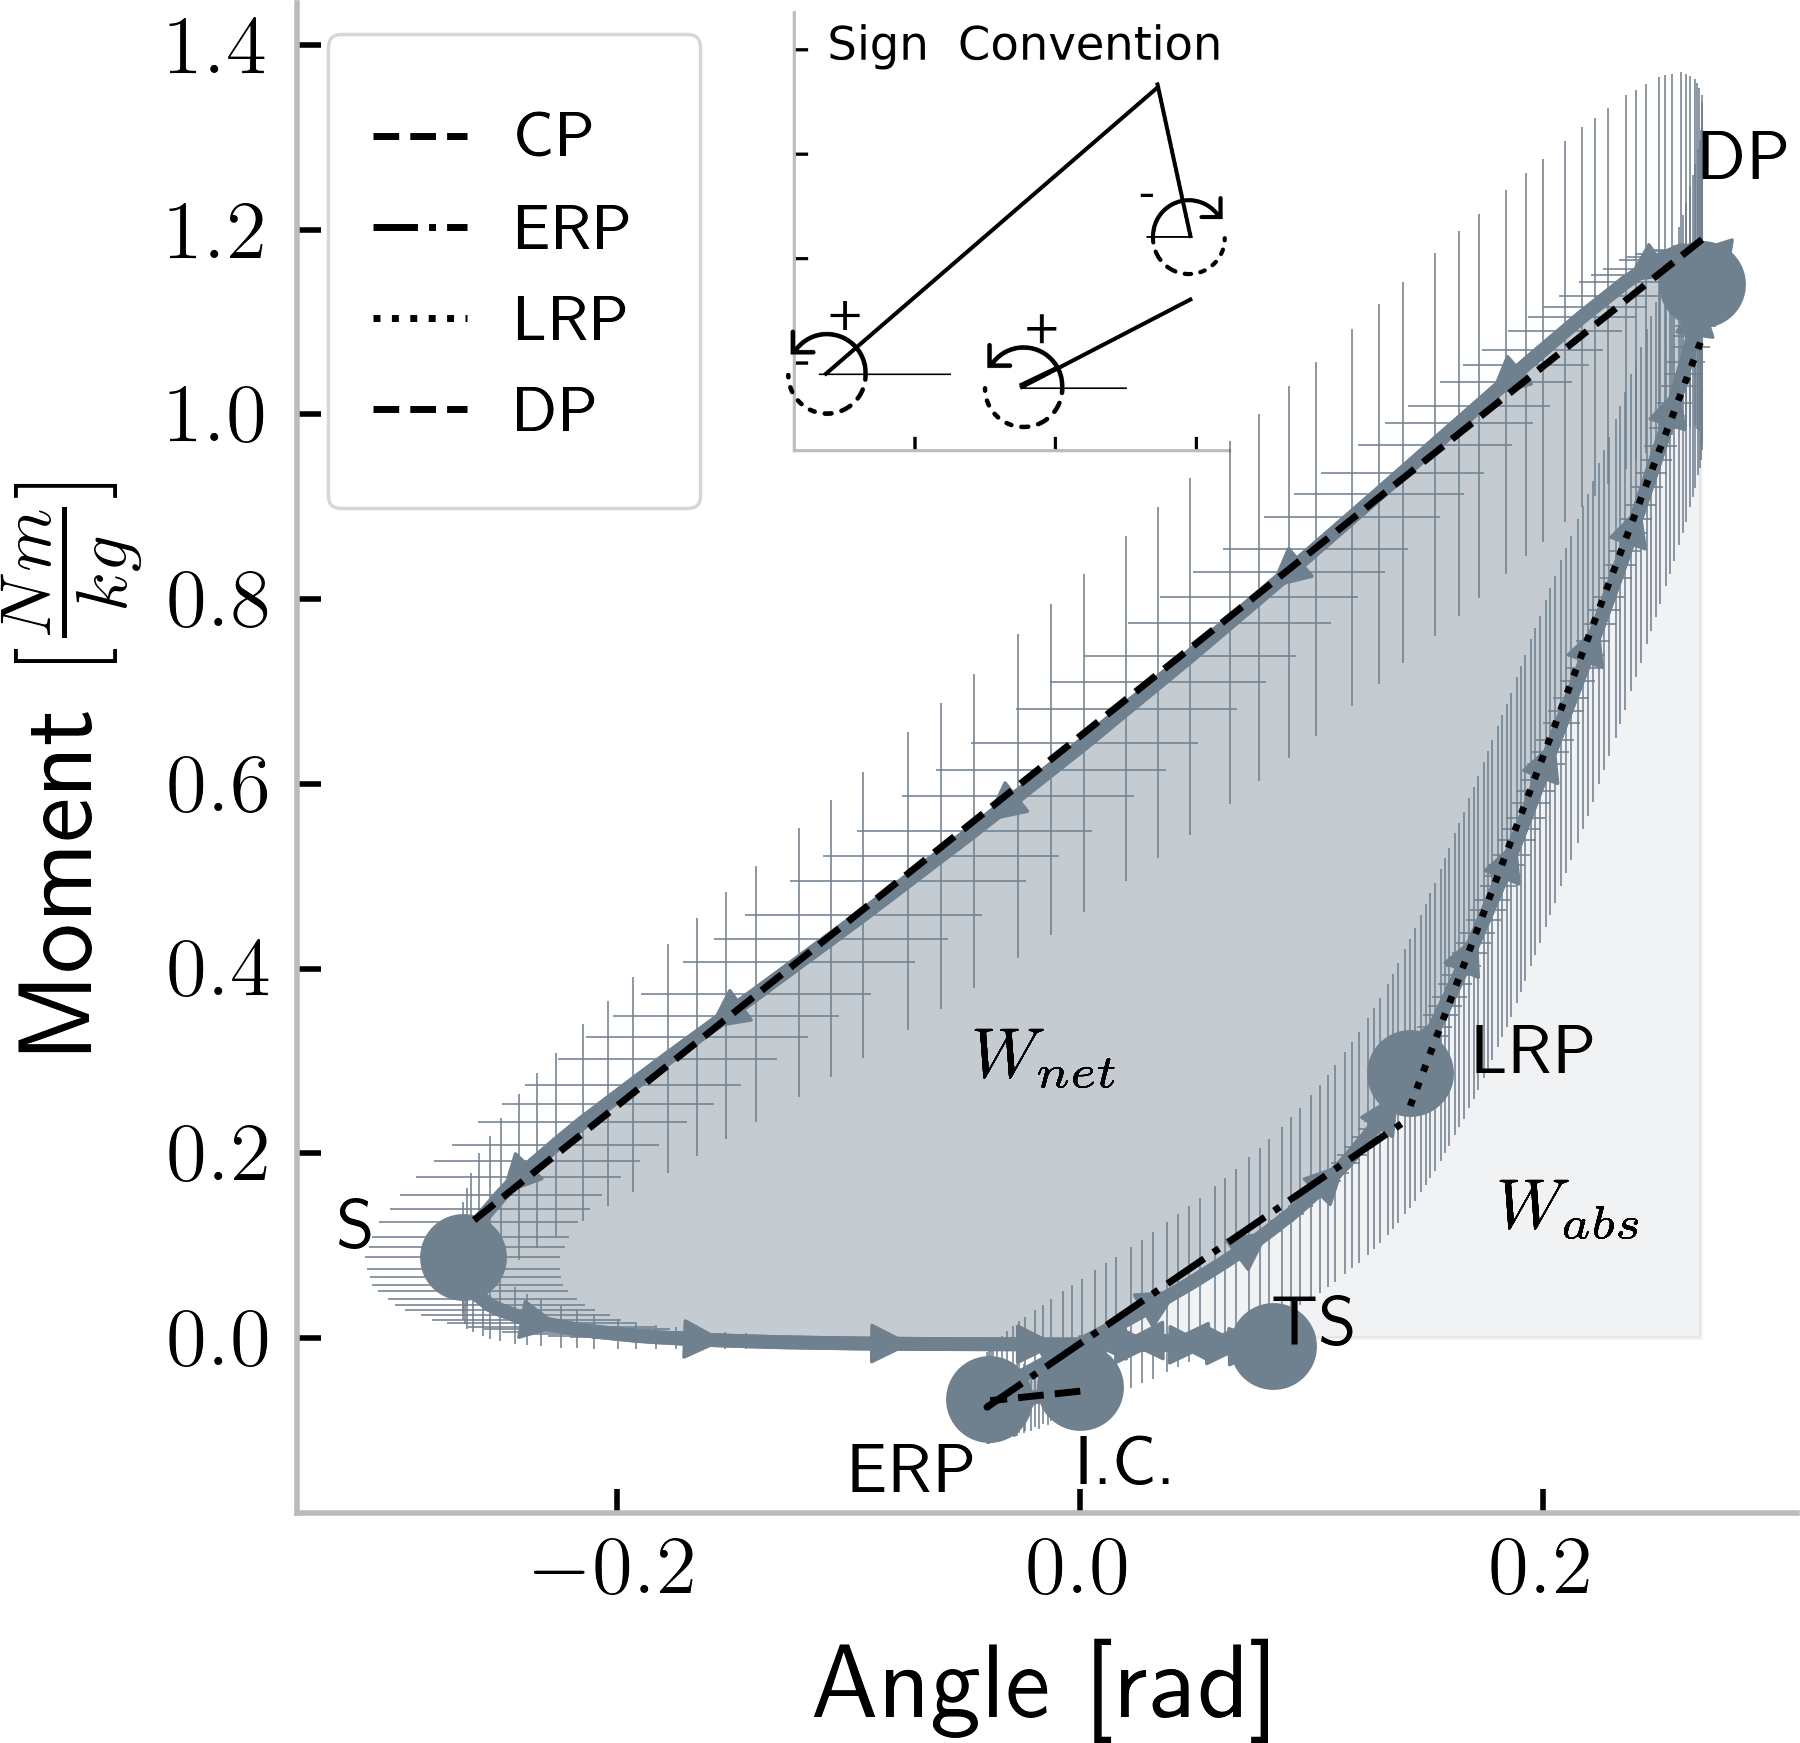
\includegraphics[scale=0.60]{Feathergraphics/general_conventions_QS.png}}
\caption{{\footnotesize Description of the Ankle DJS characteristics. Turning points represented as initiating: Contact (I.C), Early Response Phase (ERP), Late Response Phase (LRP), Descending Phase (DP), Swing (S) and Terminal Swing (TS). Regression fits: Controlled Plantar-flexion (CP), ERP, LRP and DP. Ankle DJS direction, mechanical net work ($W_{net}$), absorbed work ($W_{abs}$) and SD are shown on each DJS plot.}}
\label{fig:conventions}
\end{center}
\end{figure}

\end{frame}

%----------------------------------------------------------------
\section{Problem statement}

\subsection{Research Question and Objectives}

\begin{frame}{Identificación del problema}

\begin{block}{Problem Statement}

The recent passive prosthesis for transtibial amputees produce disorders in the dynamic parameters of the gait, owing to the absence of positive work of the limb loss. 

\end{block}
	\end{frame}

\subsection{Reseach Question}
\begin{frame}{Problem Identification}

\begin{block}{Research Question}

Which passive ankle-foot prosthesis based on cellular solids configurations, will generate the positive work needed for push-off, taking advantage of the energy lost at initial contact of the gait?

\end{block}
\begin{block}{Hipótesis}

A passive dynamic system (compound of cellular solids) within a passive ankle-foot prosthesis, configured to store energy in a controlled manner at initial contact of the early stance phase, will enable to return the stored energy after dorsiflexion phase.

\end{block}
\end{frame}

\section{Objectives}

\subsection{Objectives}
\begin{frame}{Objectives}

\begin{alertblock}{General Objective}

To suggest an ankle-foot prosthesis being able to generate - through a passive dynamic system - the positive work needed for push-off after dual-flexion phase, taking advantage of the energy lost at initial contact of the gait.

\end{alertblock}
\end{frame}


\subsection{Specific Objectives}
\begin{frame}{Objectives}

\begin{exampleblock}{Specific Objectives}

\begin{enumerate}
\item Identify biomechanical parameters and the work-loop slope of ESR prosthesis users and non-amputees aiming to obtain the ankle quasi-stiffness of both cases.

\item Obtain a preliminary model of the ankle-foot prosthesis capable of storing energy (during initial contact until late dual-flexion phase), and returning it at dorsi-flexion phase in a controlled manner through the passive dynamic system.

\item Determine detailed configurations of cellular solids that accomplish the requirements of the preliminary model.
\item Validate the dynamic model of the ankle-foot prosthesis in comparison to an ESR prosthesis. 
\end{enumerate}
\end{exampleblock}
\end{frame}


\section{Metodología y actividades}
\subsection{Metodología general}
\begin{frame}{Methodology \emph{In Silico}}{Validation process}

\begin{figure}
\centering{}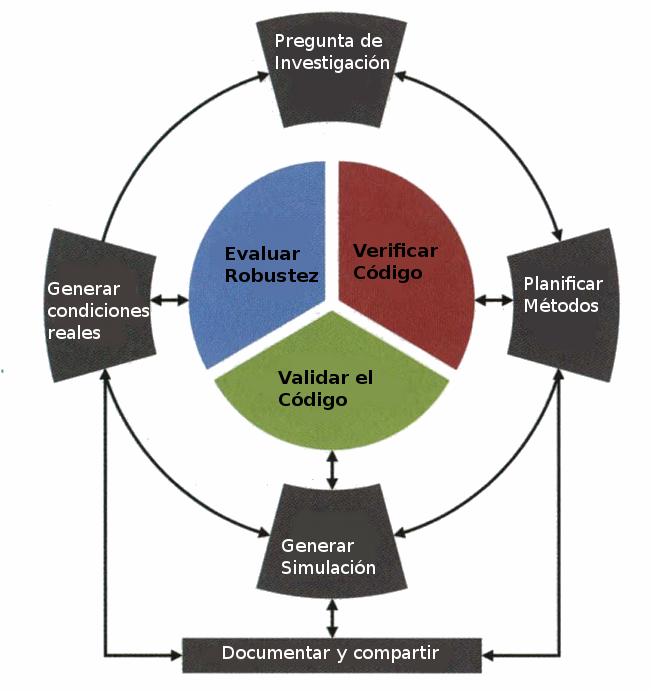
\includegraphics[scale=0.35]{Feathergraphics/verificationprocess}
\caption{{Proceso metodológico modelo \emph{In silico}. Tomado de  \cite{Hicks2014}.}}
\end{figure}

\end{frame}

\begin{frame}{Methodology \emph{In Silico}}{Computational Framework implemented.}
\begin{figure}[ht]
\begin{centering}
\begin{tikzpicture}[
    mindmap,
    every node/.style=concept,
    concept color=black!40,
    grow cyclic, text=white,
    level 1/.append style={level distance=2.2cm,sibling angle=90},
    level 2/.append style={level distance=1.8cm,sibling angle=45}, every node/.append style={scale=0.6}
    ]
  \node [root concept] {\Large{Python}} % root
    child [concept color=myblue] { node {Modelo biomecánico}
      child { node {Opensim} } 
      child { node {BTK} }
    }
    child [concept color=myblue] { node {Simulador FEM}
      child { node {Elmer} }
    }
    child [concept color=myblue] { node {Modelo multicuerpo}
      child { node {Simbody} }
      child { node {Pydy} }
    }
    child [concept color=myblue] { node {Visualizadores}
      child { node {VTK} }
      child { node {Paraview} }
    };
\end{tikzpicture}
%\caption{\label{Marco-computacional} Marco computacional \emph{Open-source} de la metodología tentativa a implementar en el proyecto.}
\end{centering}
\end{figure}

\end{frame}

\begin{frame}{Development of the 1st Objective}
\begin{columns}[t]


\column{65 mm}
\begin{block}{}
{\footnotesize{}}

\begin{figure}
\begin{centering}
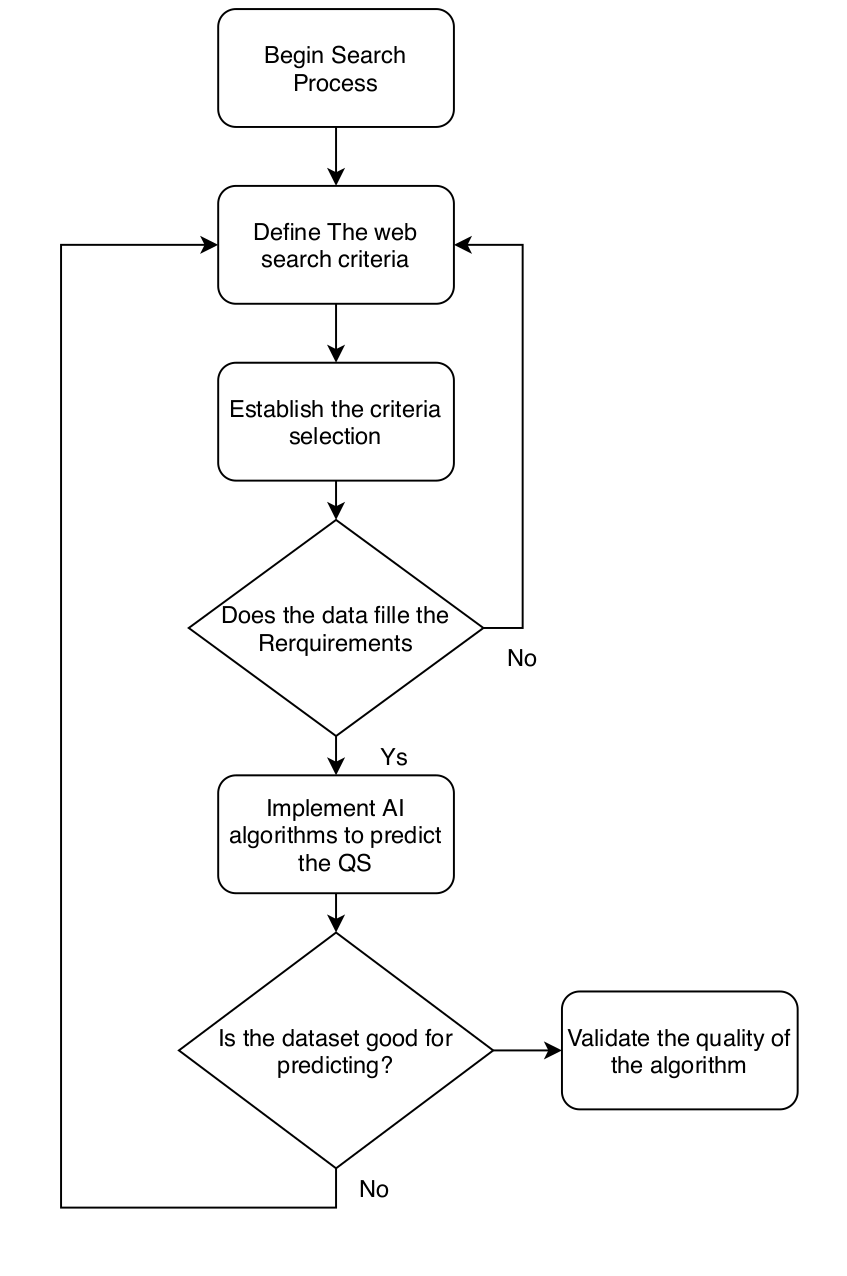
\includegraphics[scale=0.12]{Feathergraphics/Ob1flowchart}
\par\end{centering}
\caption{{\scriptsize{}Execution flowchart for Obj. 1}}
\end{figure}

\end{block}

\column{50 mm}
\begin{exampleblock}{}

\begin{figure}
\begin{centering}
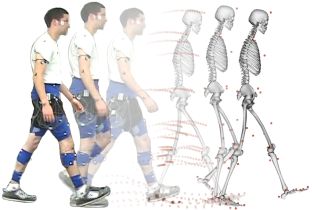
\includegraphics[scale=0.40]{Feathergraphics/labToModel}
\par\end{centering}
\caption{{\scriptsize{}Marker Experiments taken from Horst}}
\end{figure}
\end{exampleblock}
\end{columns}
\end{frame}

\begin{frame}{Methodology \emph{In Silico}}{Validation process}

\begin{figure}
\centering{}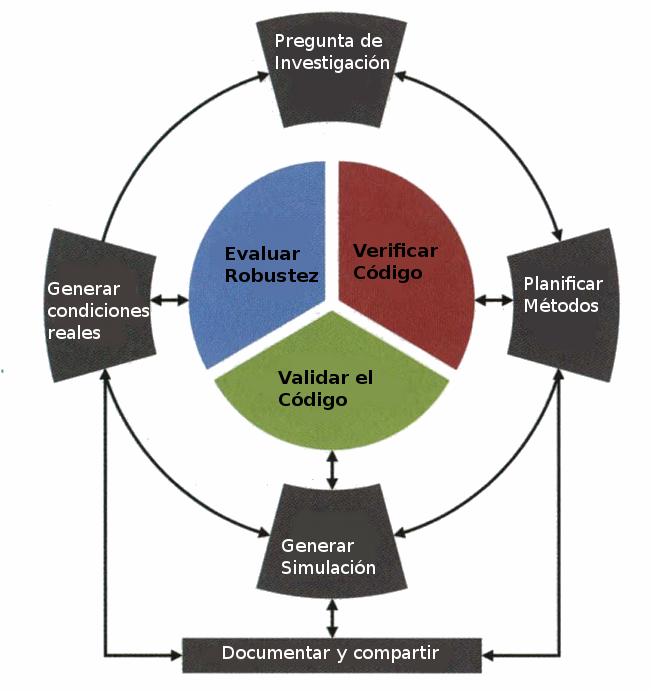
\includegraphics[scale=0.35]{Feathergraphics/verificationprocess}
\caption{{Proceso metodológico modelo \emph{In silico}. Tomado de  \cite{Hicks2014}.}}
\end{figure}


\end{frame}

\begin{frame}
    \begin{figure}[!ht]
\centering
    \subfloat[]{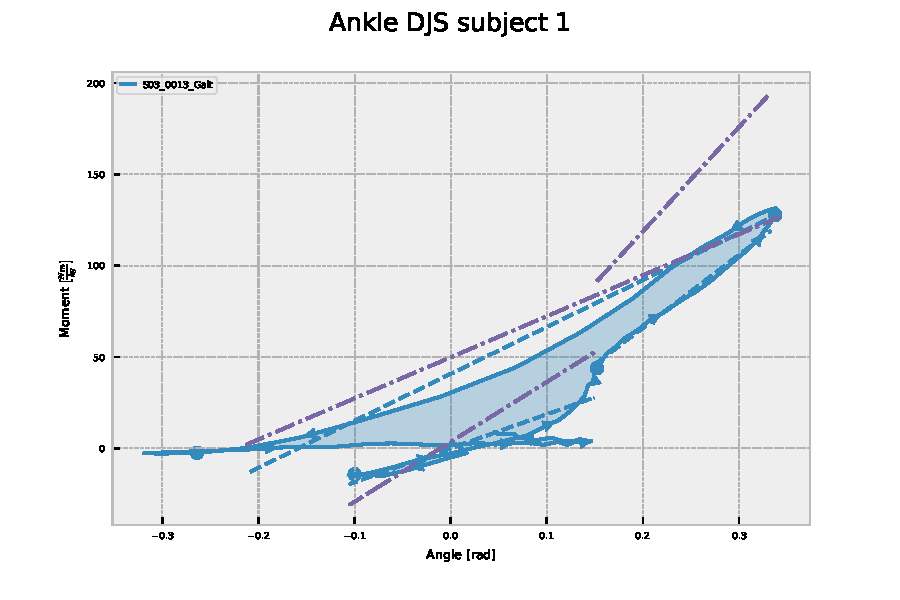
\includegraphics[width=0.3\linewidth]{Feathergraphics/compregressorsample6.pdf}}
    \subfloat[]{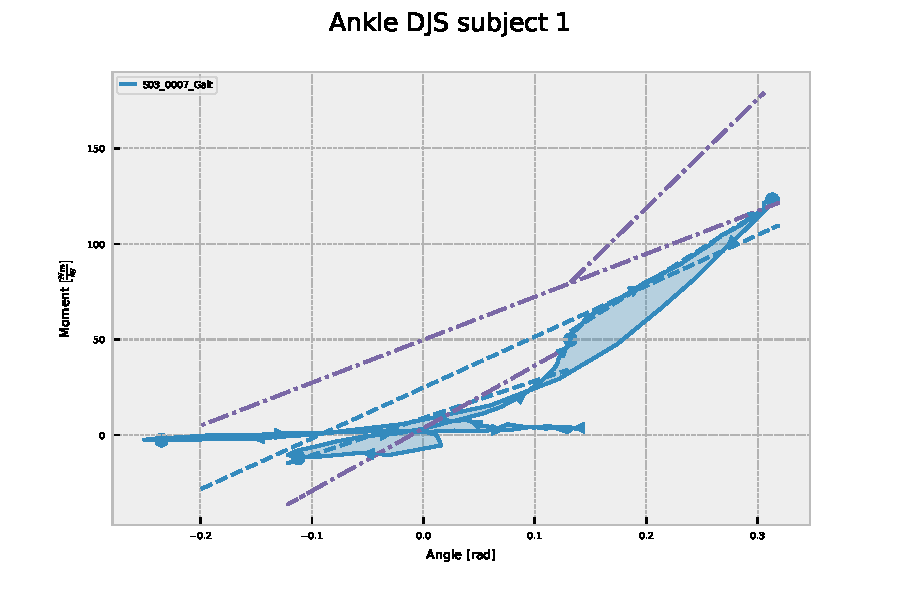
\includegraphics[width=0.3\linewidth]{Feathergraphics/comp_regressor_sample_5.pdf}}
    \subfloat[]{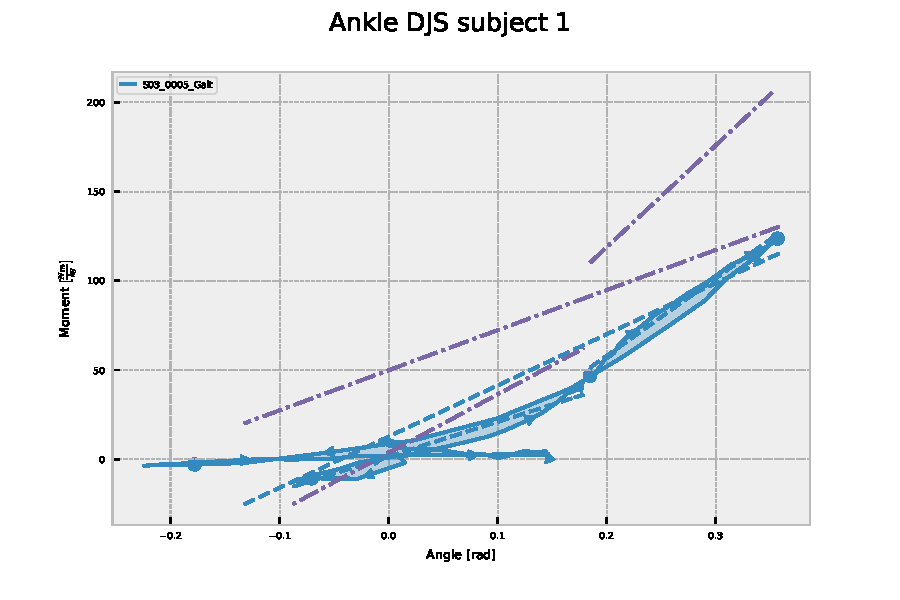
\includegraphics[width=0.3\linewidth]{Feathergraphics/comp_regressor_sample_4.pdf}}
    
    \subfloat[]{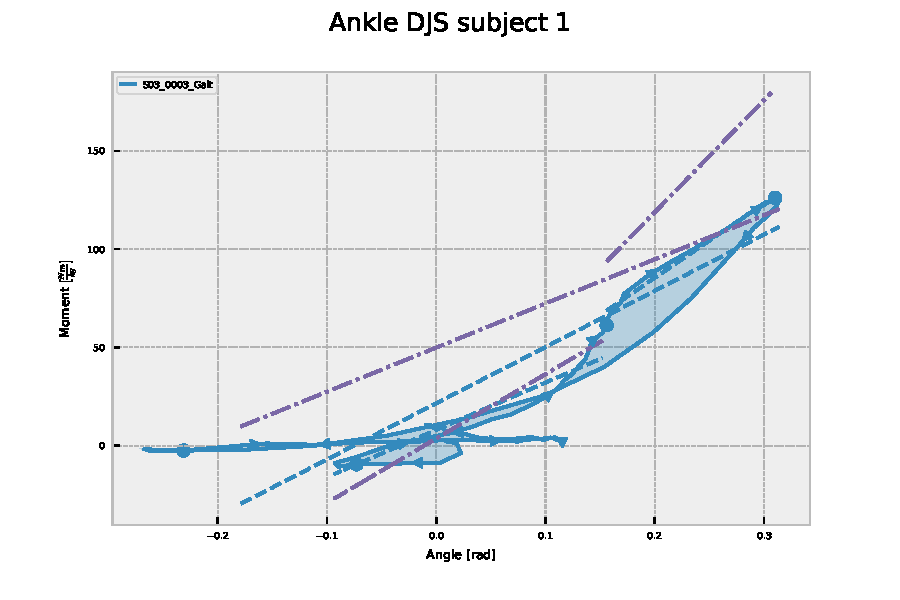
\includegraphics[width=0.3\linewidth]{Feathergraphics/comp_regressor_sample_3.pdf}}    
    \subfloat[]{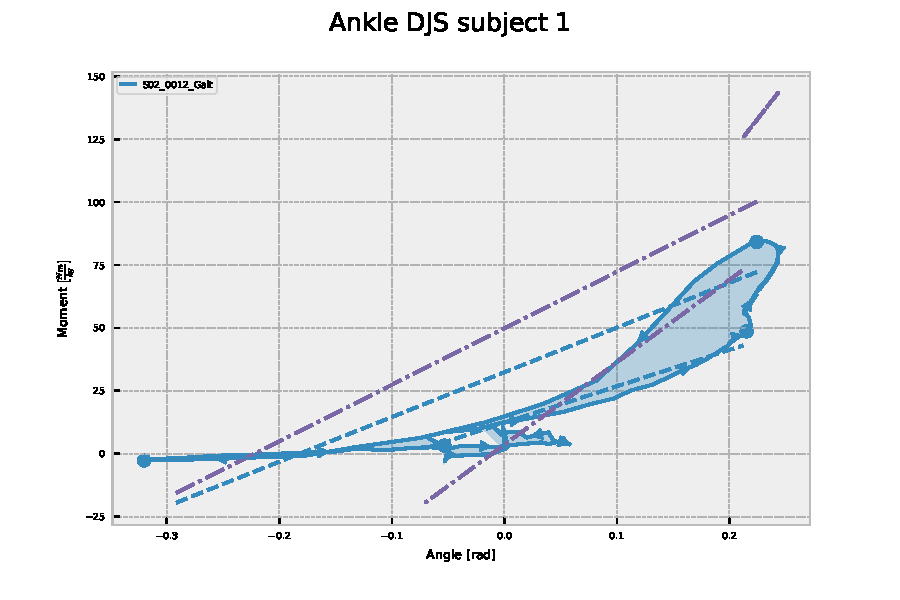
\includegraphics[width=0.3\linewidth]{Feathergraphics/comp_regressor_sample_2.pdf}}
    \subfloat[]{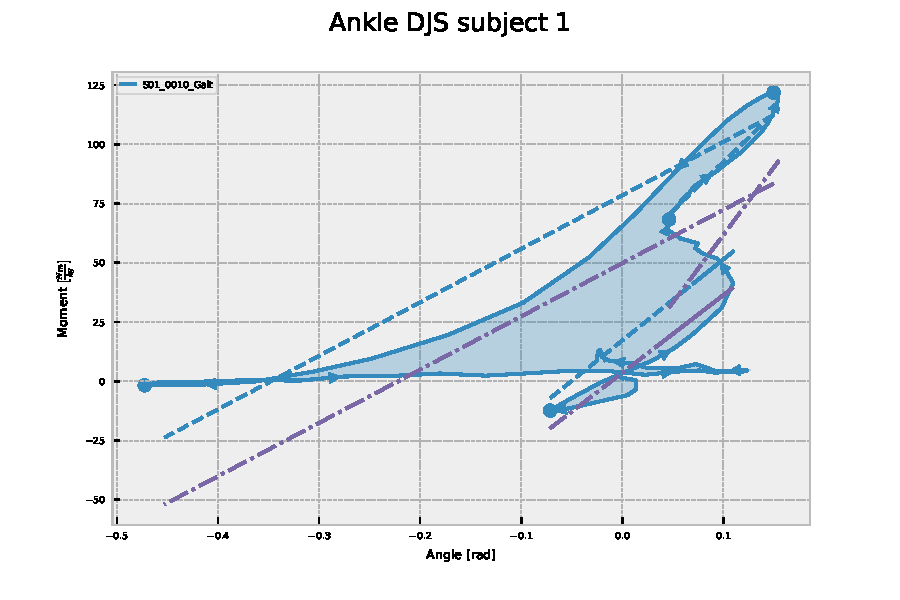
\includegraphics[width=0.3\linewidth]{Feathergraphics/comp_regressor_sample_1.pdf}}
\caption{comparison of the predicted feature vs testing sample}
    \label{fig:outputsamples}
    \end{figure}
\end{frame}

\begin{frame}{Sensitivity Analysis}
    \begin{figure}[!ht]
\centering
    \subfloat[]{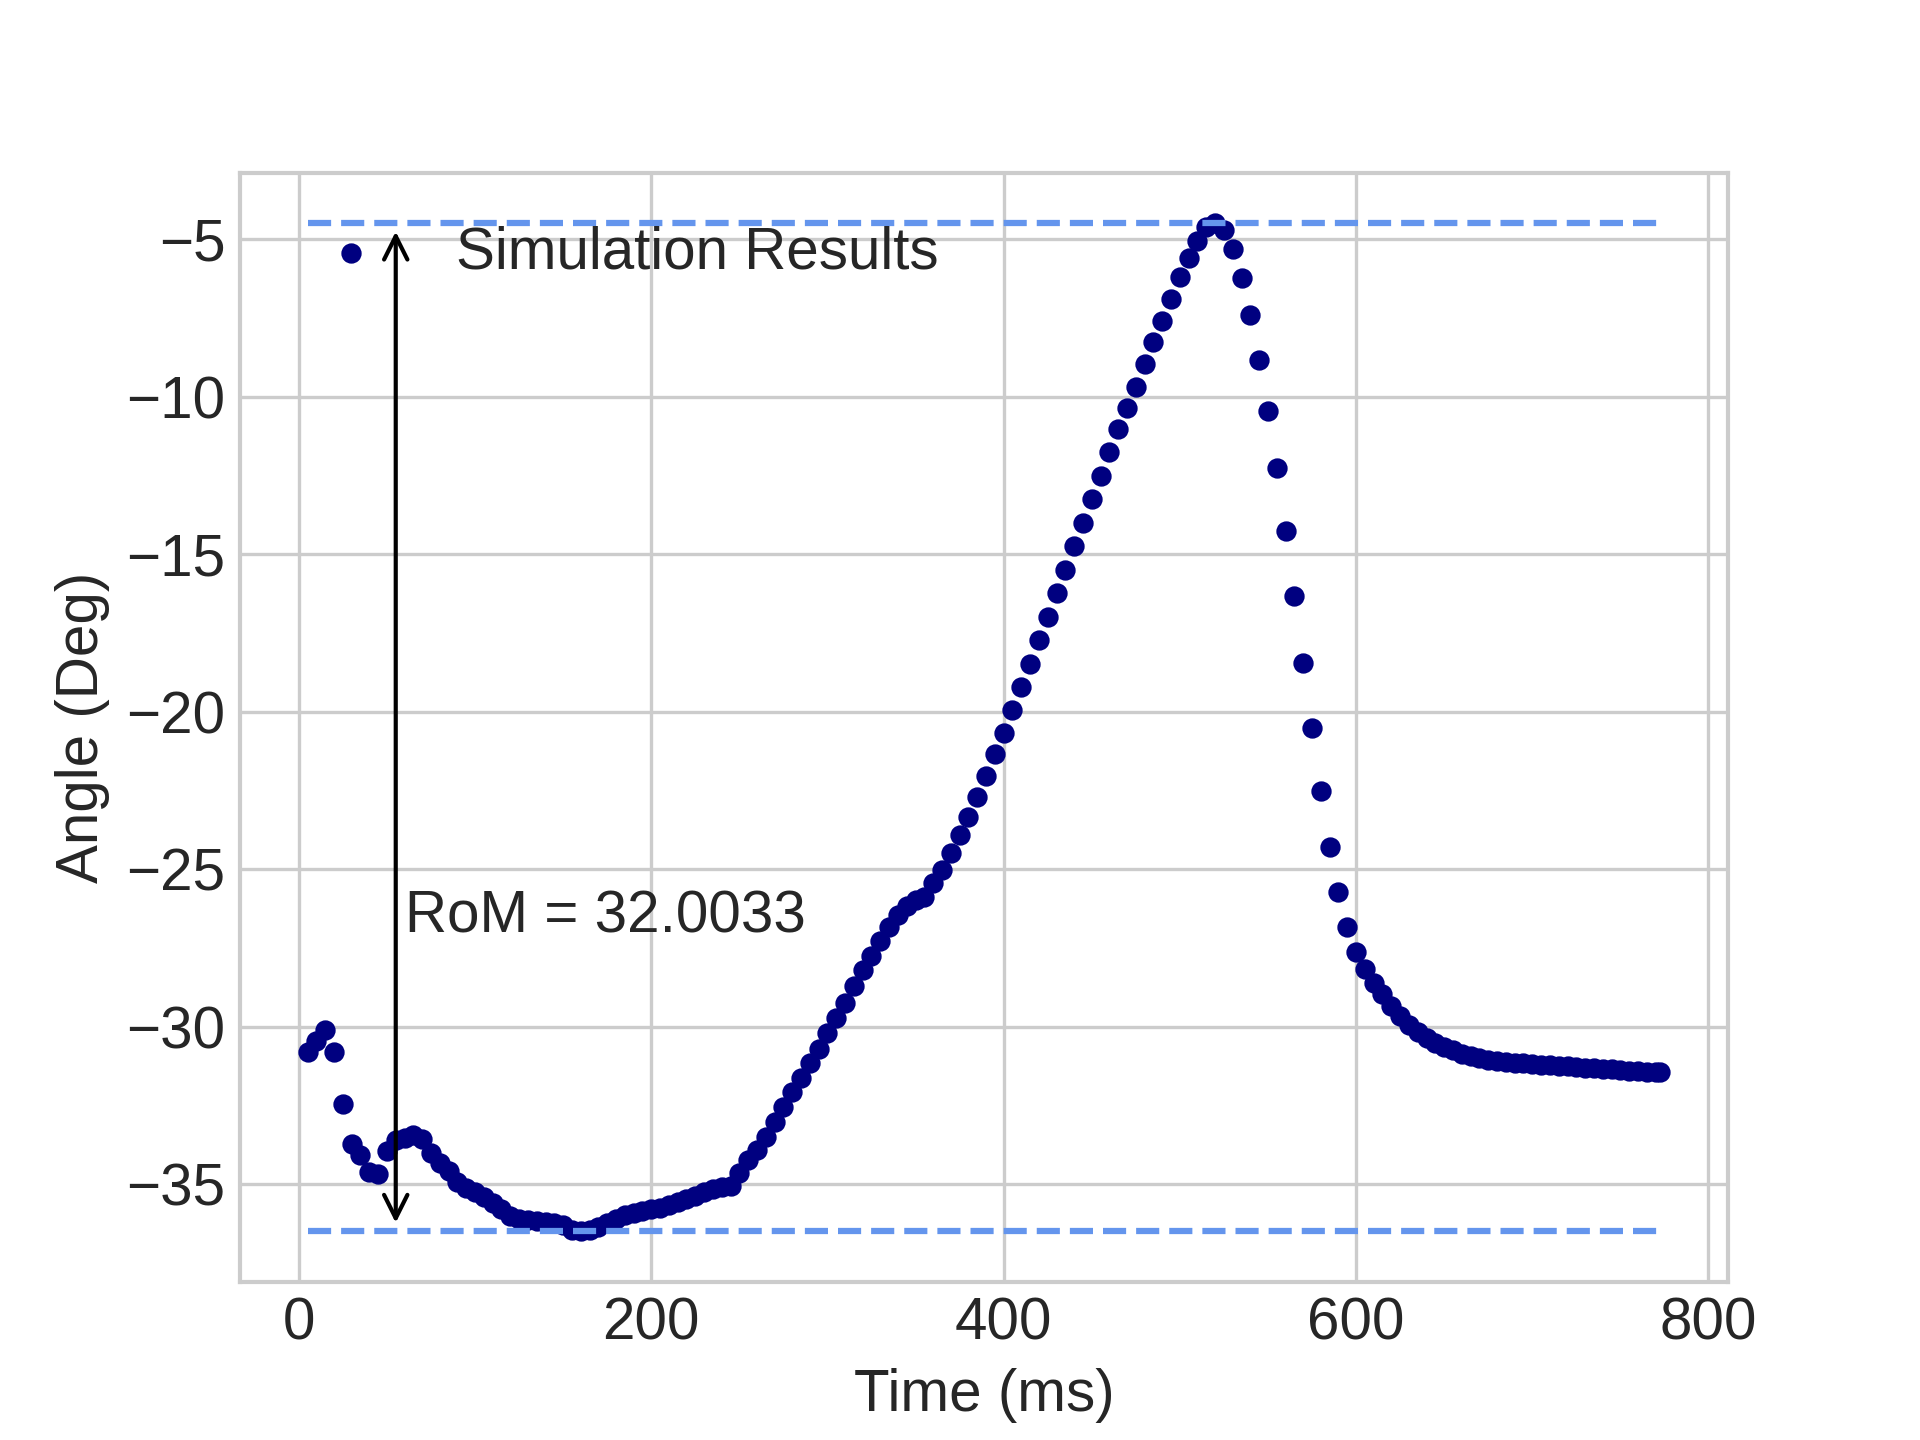
\includegraphics[width=0.3\linewidth]{Feathergraphics/angle_RoM.png}}
    \subfloat[]{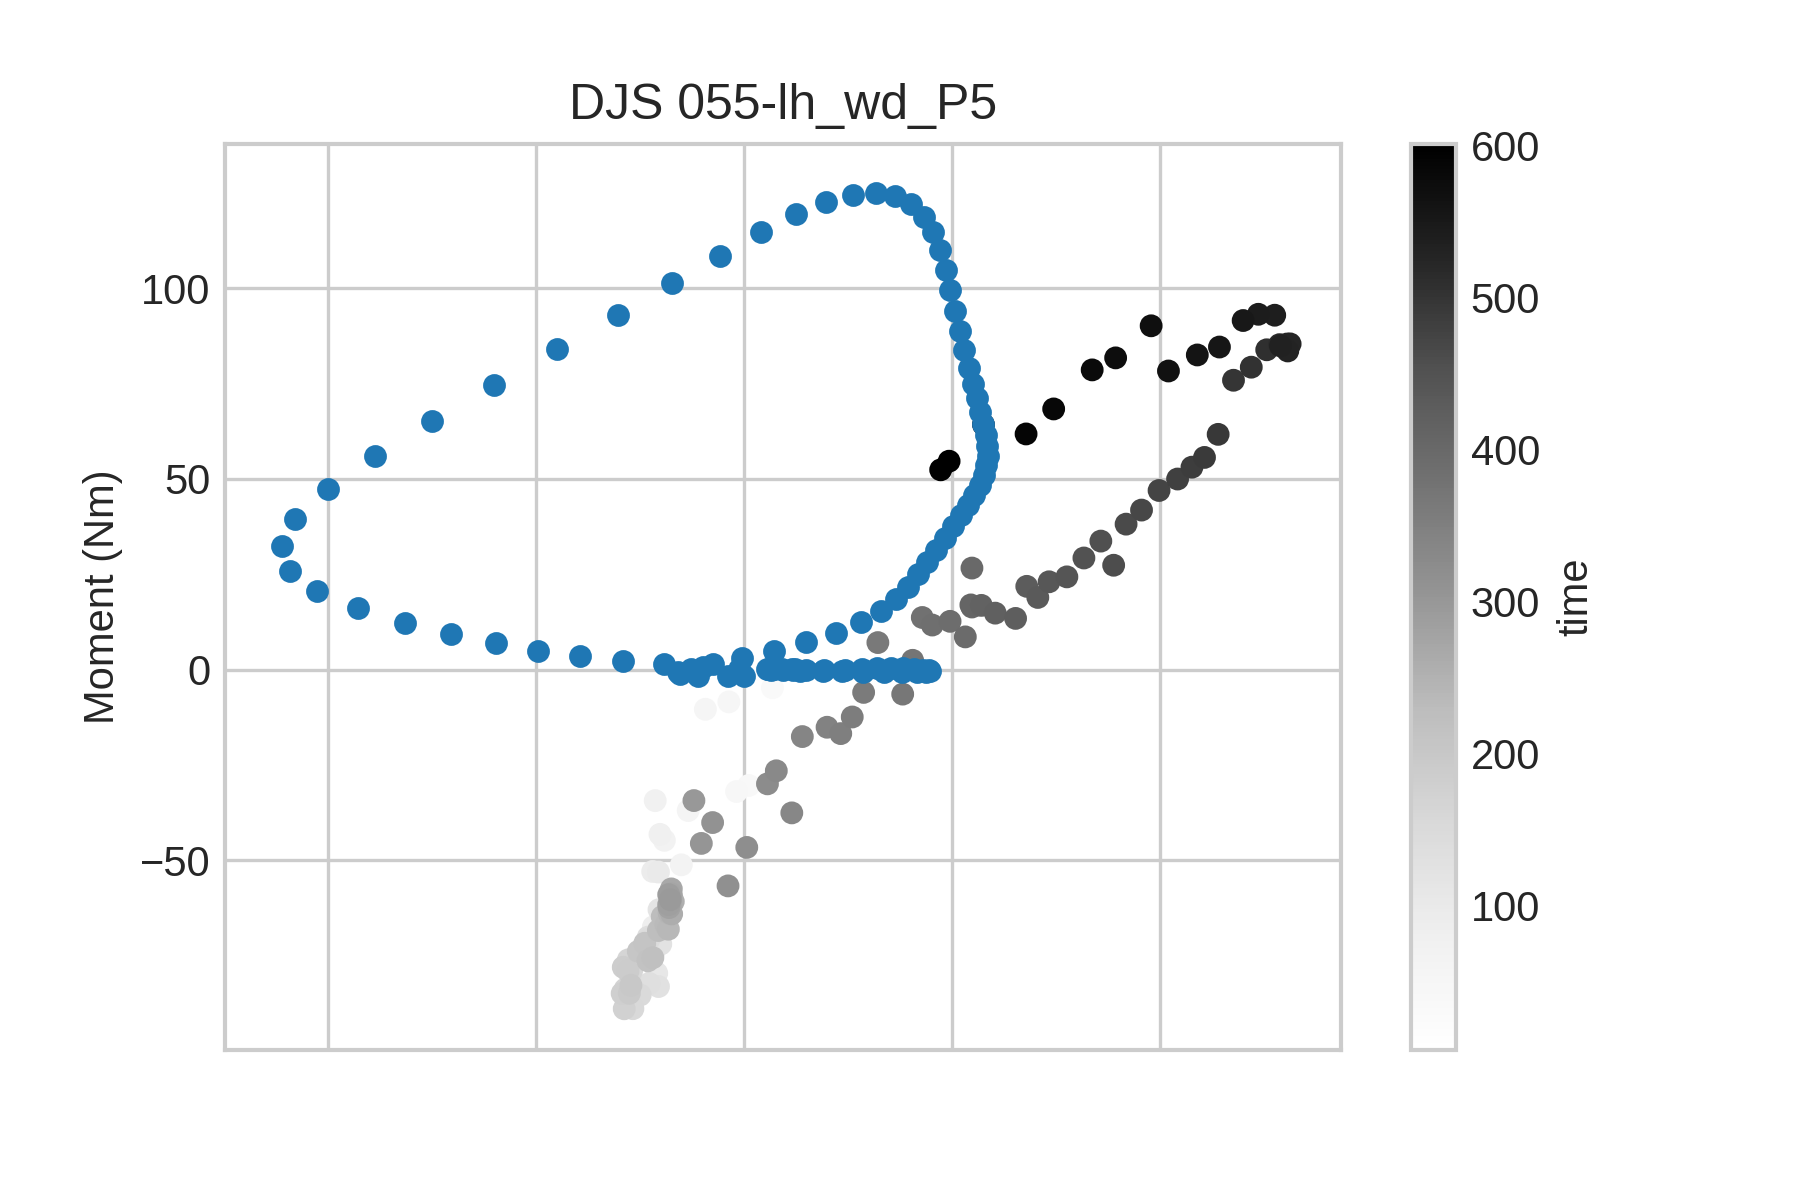
\includegraphics[width=0.3\linewidth]{Feathergraphics/QS.png}}
    
    \subfloat[]{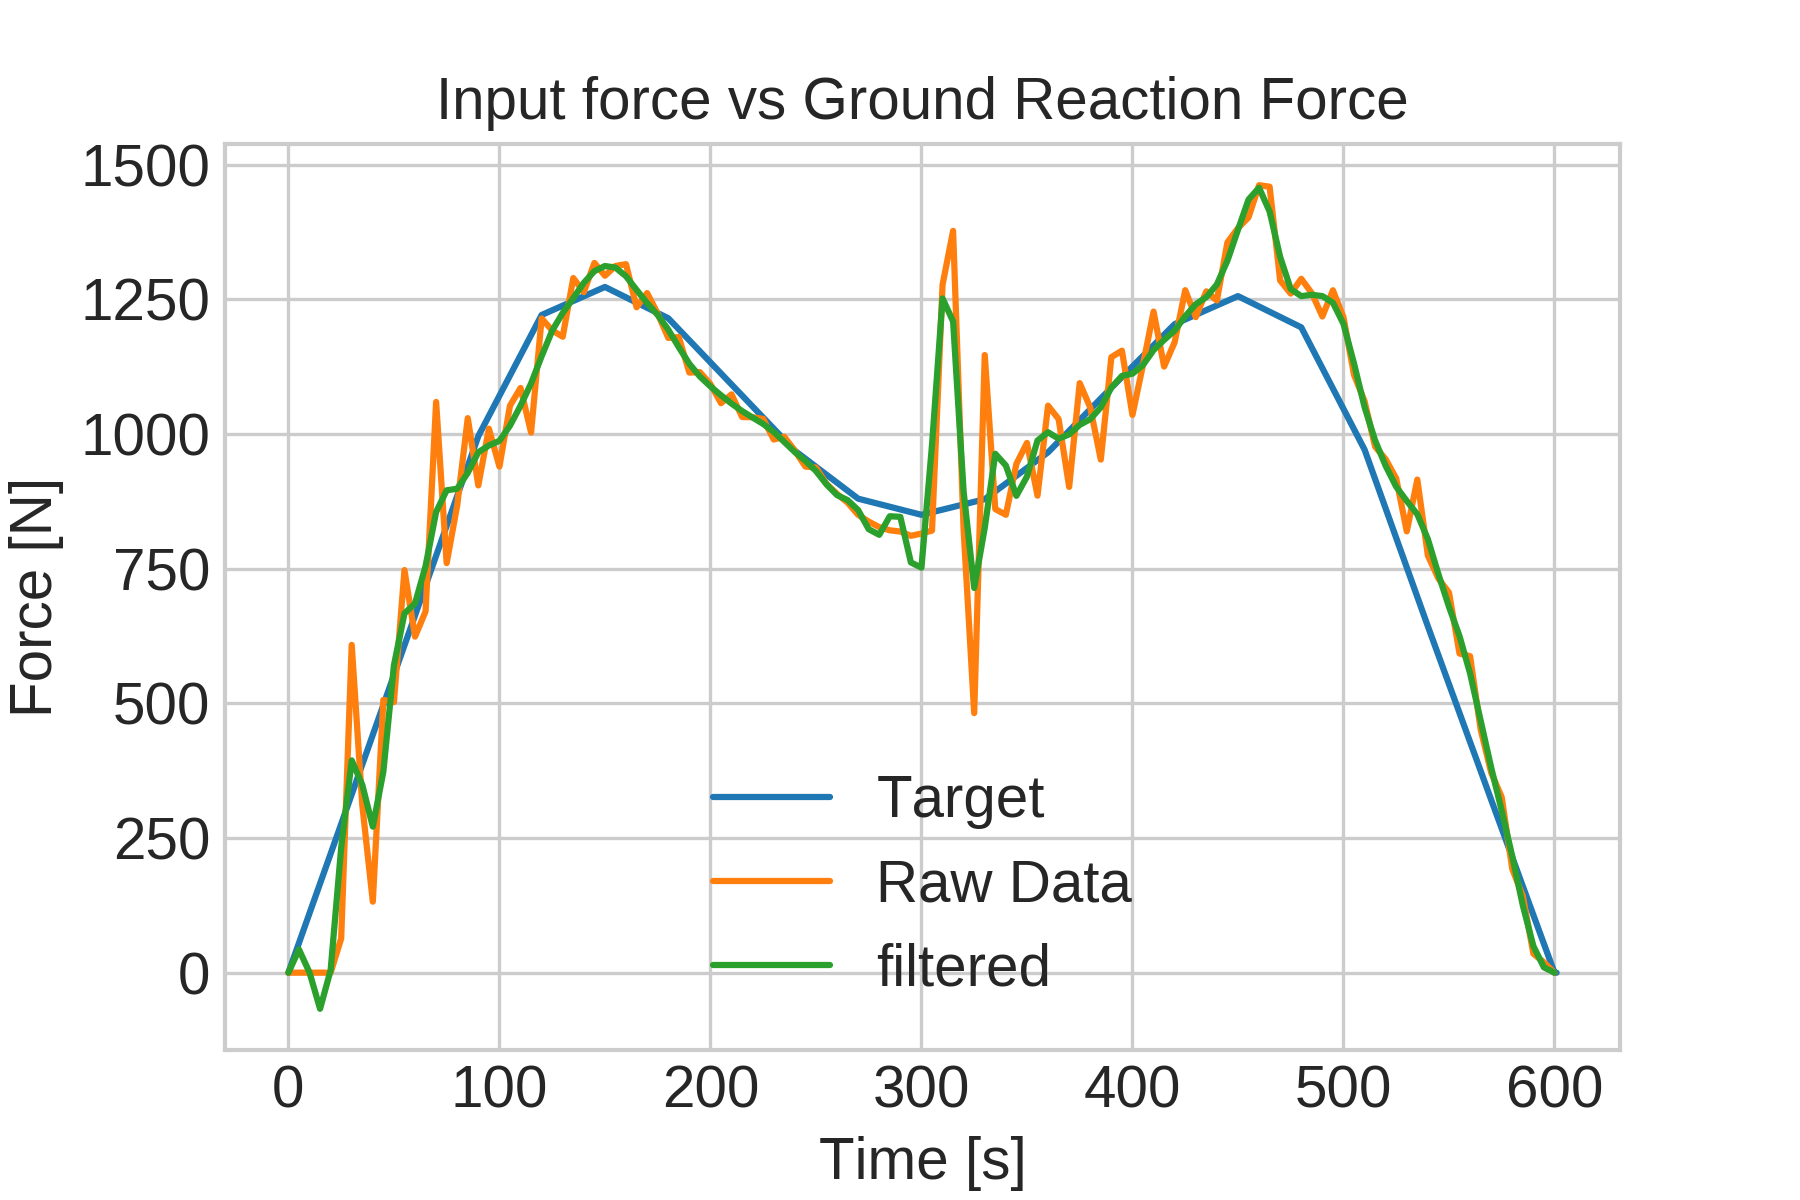
\includegraphics[width=0.3\linewidth]{Feathergraphics/ErrorGRF.png}}
    \subfloat[]{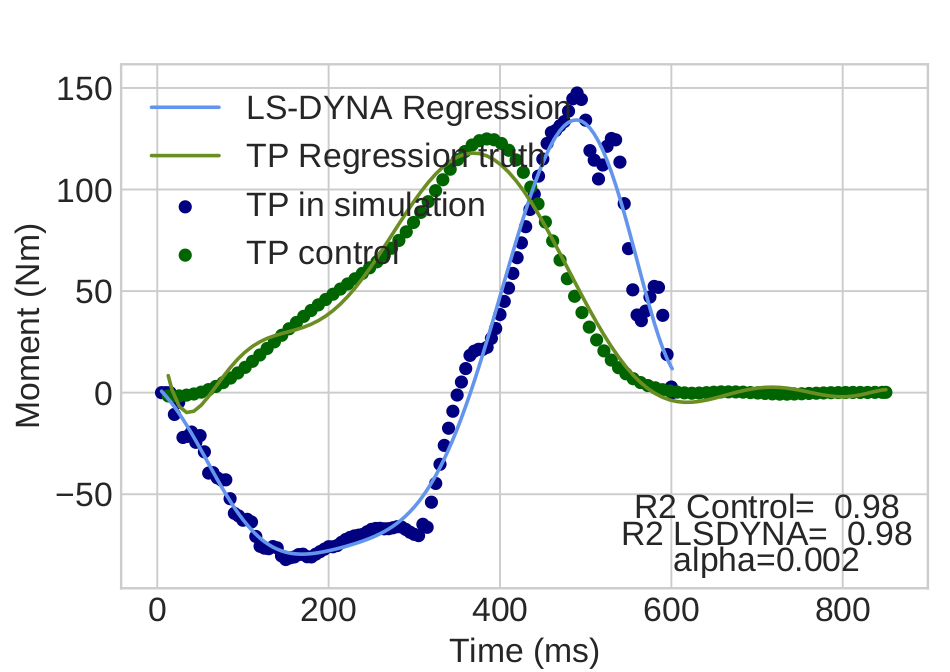
\includegraphics[width=0.3\linewidth]{Feathergraphics/ErrorMom.png}}

\caption{Variable outputs}
    \label{fig:SAnalysis}
    \end{figure}
\end{frame}

\begin{frame}{Thickness analysis}
\begin{figure}
\centering{}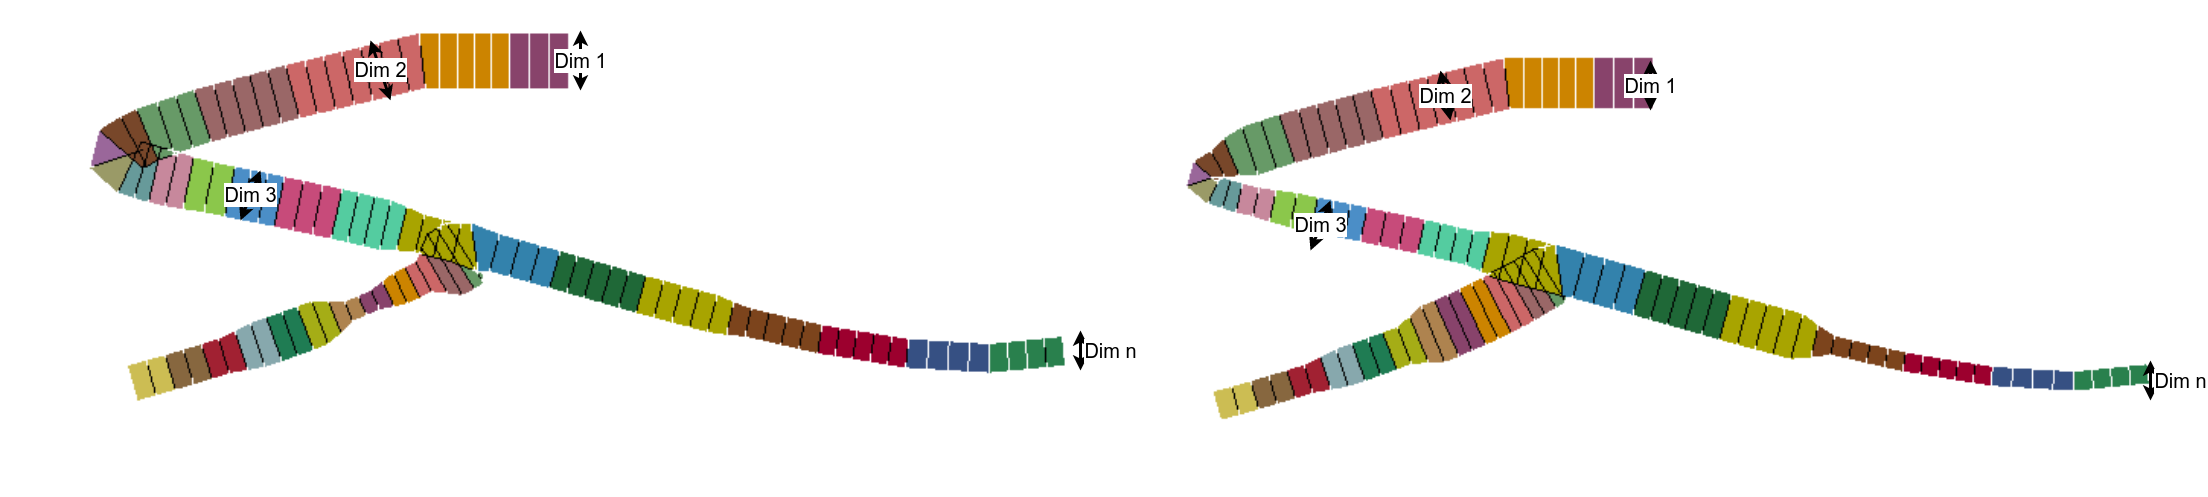
\includegraphics[scale=0.15]{Feathergraphics/Thickness_variationAF.png}
\caption{Thickness Varation samples}
\end{figure}
\end{frame}

\begin{frame}{Shape Optimization analysis}
\begin{figure}
\centering{}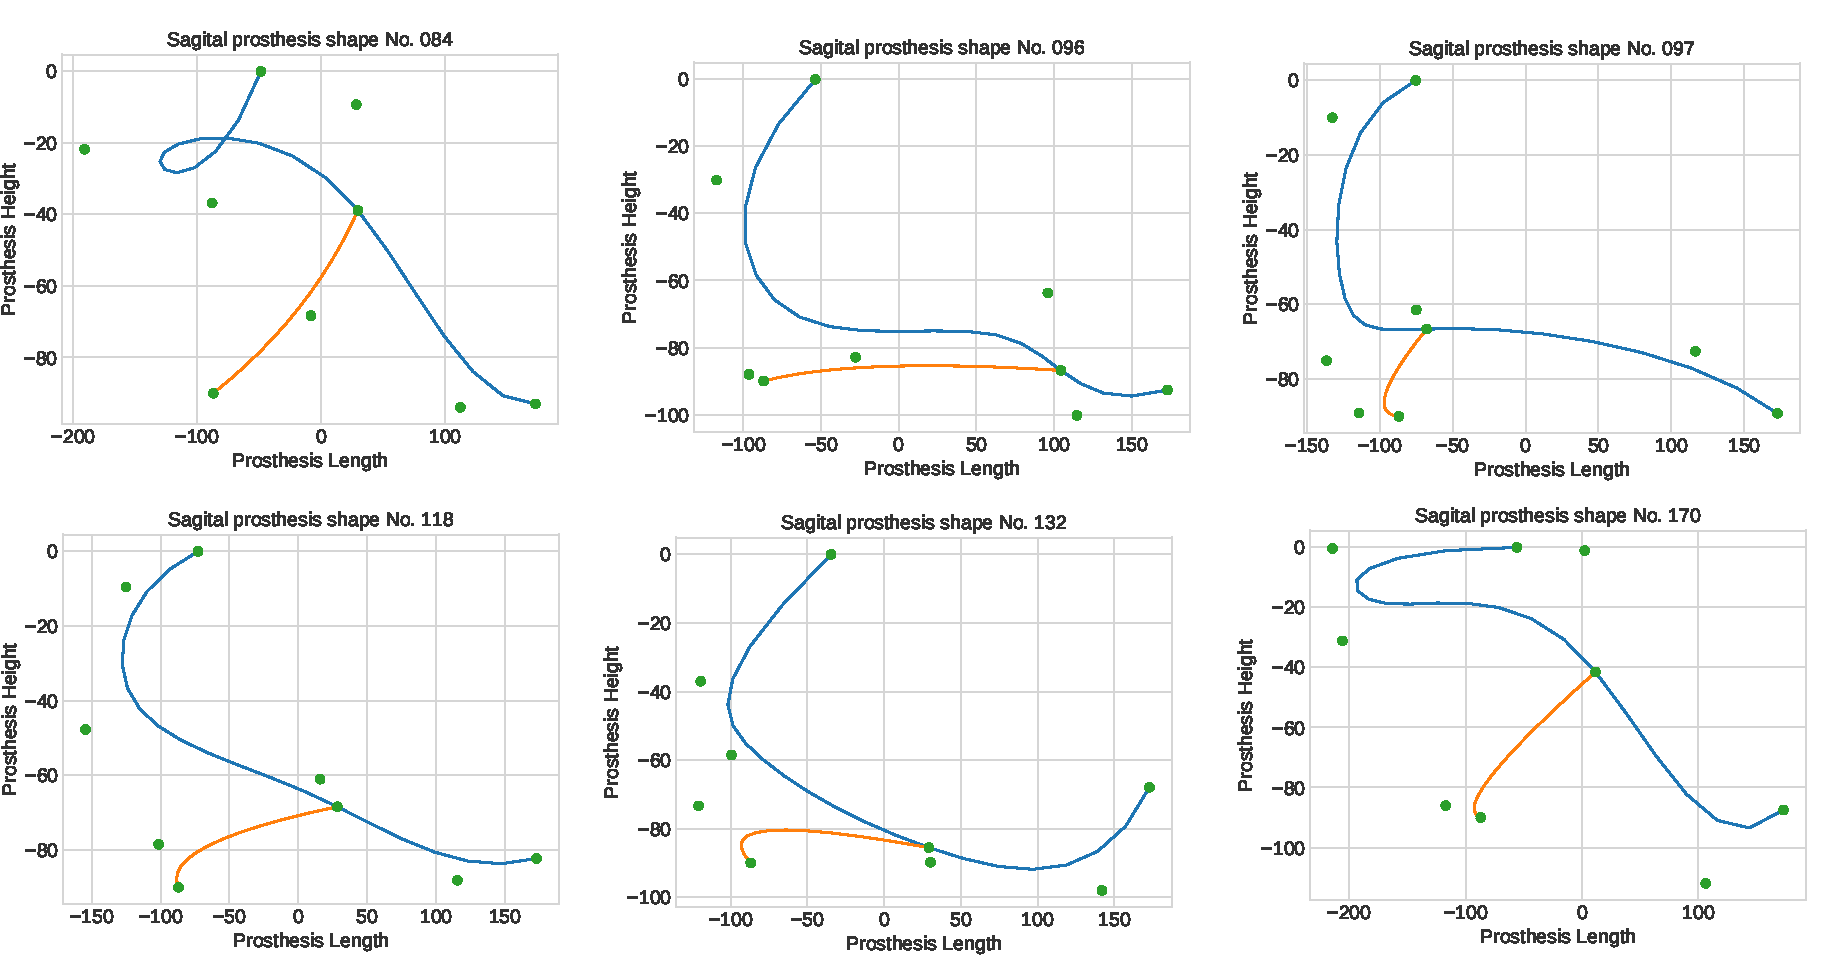
\includegraphics[scale=0.70]{Feathergraphics/shapesAF.png}
\caption{Thickness Varation samples}
\end{figure}
\end{frame}
%\backupbegin
\begin{frame}[allowframebreaks]{Bibliografía}

%-------------------------------------------------------
\bibliographystyle{IEEEtran}
\tiny{\bibliography{Proposal.bib,patents.bib}}
\end{frame}
%\backupend

{\BiOM
\begin{frame}[plain,noframenumbering]
  \finalpage{Thank You!\\\emph{enprietop@unal.edu.co}}
\end{frame}}
% Appendix

\end{document}